\chapter{The Extended Roofline Model}
\section{The Conventional Rooflne Model}

The Roofline model estimates the performance of an application running on a multi-core processor by exploring the hardware limitations. The performance bottlenecks are characterised as computation and data transfer. Assuming a scenario that there are $B$ Gbytes of data transfer from the memory to the CPU. The processor has the peak performance of $P_{max}$ GFlops/s. The memory provides the maximal bandwidth of $BW$ GB/s. Assuming the processor finished $F$ floating-point operations and there is perfect overlap between computation and data transfer, the data transfer time is $B/BW$ seconds, and the processor takes $F/P_{max}$ seconds to finish all the operations \cite{12}. The total execution time is 
\begin{equation}
T = \max \begin{cases}
{F/(P_{max})}\\
{B/BW}
\end{cases}
\end{equation}
Since the performance is measured as GFlops/s, both sides of the equation can be divided by $F$ and the result is reciprocated. The attainable performance is hereby 
\begin{equation}
P = min\begin{cases}
{P_{max}}\\
{I*BW}
\end{cases}
\end{equation}

The peak performance of the processor and the peak memory bandwidth are hardware-specific given by the vendor. The realistic maximal memory bandwidth can be measured by the STREAM benchmark \cite{12}. The attainable performance is visualised as a function $P$ with one variable  $I = F/BW$. $I$ is defined as the arithmetic intensity or operational intensity. 

\begin{figure} [h] %hier können noch Positionierungswünsche angegeben werden
	\centering   % Alles weitere zentrieren
	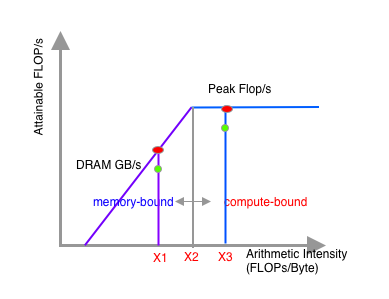
\includegraphics[width=9cm]{pictures/fig3.2}
	\caption{The Roofline model}
	\label{fig3.2}  %Reihenfolge ist wichtig! Immer erst \caption{} dann \label{}
\end{figure}

Figure 3.1 illustrates the Roofline the attainable performance depending on the arithmetic intensity. The x-axis is the arithmetic intensity and the y-axis is the attainable peak performance with logarithmic scales. The arithmetic intensity describes how many operations a kernel takes per data transfer. To determine whether an application is compute-bound or memory-bound, one simply compares the arithmetic intensity with the machine balance, which is the ratio of the peak performance to the peak bandwidth $P_{max}/Bandwidth$. The machine balance is hardware specific.

The arithmetic intensity $X_1$ is less than the machine balance $X_2$, which implies that the kernel spends more time on data transfer than computation. Therefore, the application is memory-bound. Its maximal attainable performance is $X_1 * BW$, which sits on the bandwidth ceiling (red dot for $X_1$). For some applications, the measured memory bandwidth does not necessarily reach the maximum, in this case, the actual performance is below the ceiling (the green dot for $X_1$). 

The arithmetic intensity $X_3$ is greater than the machine balance $X_2$, as a result, it is compute-bound. The attainable performance is $P_{max}$, which sits on the computational ceiling (red dot for $X_2$). In reality, the processors do not always attain the peak FLOP/s. For this case, it is represented by the green dot for $X_3$, which is below the computational ceiling.

\section{The Hierarchical Roofline Model}
%\begin{figure} [h] %hier können noch Positionierungswünsche angegeben werden
%	\centering   % Alles weitere zentrieren
%	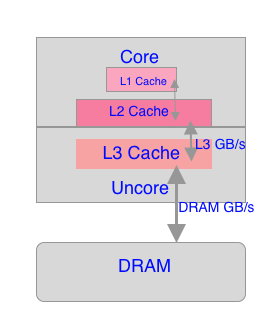
\includegraphics[width=4cm]{pictures/fig3.3}
%	\caption{Memory hierarchy}
%	\label{fig3.3}  %Reihenfolge ist wichtig! Immer erst \caption{} dann \label{}
%\end{figure}

Chapter 3.1 introduces the naive performance analysis on the kernel and DRAM. In reality, the Roofline model must be implemented on the hierarchical memory architecture, which is introduced in Chapter 2.1. In hierarchical memory architecture, different levels of memory have their individual bandwidths. As a result, each level has different machine balances. The data movement is also different for each level because applications have locality in a memory level. Therefore, it is important to construct the Roofline model for each memory level. This work focuses on the L3 cache and DRAM because their performances are affected by the uncore frequency. The L1 and L2 caches are located in the core area and their performances are affected by the core frequency. Two arithmetic intensities are calculated, one is the arithmetic intensity of the L3 cache, which is based on the data transfer between core and L3 cache; the other is the arithmetic intensity of DRAM, which is based on the data transfer between the processor and DRAM. 


\subsubsection{Bandwidth Ceilings}

Figure 3.2 (a) shows the Roofline function with two memory levels namely L3 cache and DRAM. The red line and the purple line represent the bandwidth ceilings for the L3 cache and DRAM respectively. Since the maximal L3 bandwidth is much higher than the DRAM. The machine balance of the L3 cache is smaller than DRAM. Assuming an application has the same measured intensities for both L3 and DRAM, the maximal attainable performance of L3 is higher than the DRAM's. As a result, the bandwidth ceiling of the L3 cache is always above the one of DRAM. 

In the hierarchical Roofline model, there exist several different arithmetic intensities. This indicates the performance bounds may be different for each memory level. In Figure 3.2 (a), the arithmetic intensity of the L3 cache $I_1$ is greater than the machine balance while the arithmetic intensity of DRAM $I_2$ is less than the machine balance. In this case, the performance is the minimum of those bound. This means it is bound to the minimal attainable FLOP/s. Since  $I_2 * BW_{DRAM}<I_1 * BW_{L3}$, the application is bound to DRAM.

\begin{figure}
  \centering
  \subfigure[L3 vs. DRAM]{
    \label{fig:subfig:a} %% label for first subfigure
    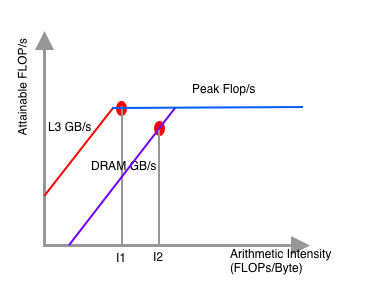
\includegraphics[width=2.9in]{pictures/fig3.4.png}}
  \hspace{0.000001in}
  \subfigure[Without SIMD or ILP]{
    \label{fig:subfig:b} %% label for second subfigure
    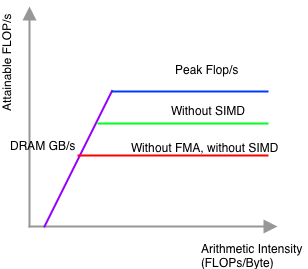
\includegraphics[width=2.5in]{pictures/fig3.5.png}}
  \caption{The hierarchical Roofline model}
  \label{fig:subfig} %% label for entire figure
\end{figure}

%In other word, the application is memory-intensive if one of the arithmetic intensities suggests memory bound, it is compute-intensive if both of the arithmetic intensities suggest compute bound. In figure 3.4 since $I_2 * bandwidth_{DRAM}<I_1 * bandwidth_{L3}$, the application is bound to memory.
\subsubsection{Computational Ceilings}
The peak Flop/s in Figure 3.2 (b) represents the theoretical upper bound of performance. In reality, applications do not always perform that well. There are several factors that affect the performance such as Single Instruction Multiple Data and Fused Multiply-Add instruction set when it comes to compute-bound situations. Those performance hindrances are mapped to the computational ceilings in Figure 3.2 (b).

\textit{Single Instruction Multiple Data (SIMD)}\\
SIMD is a method that allows a single instruction to process multiple data. SIMD has significant advantages against scalar operations on the array or vector data. Figure 3.4 presents the difference between SIMD and scalar operations. SIMD only needs one add instruction to operate the array addition. The scalar operation takes four add instructions to finish the task. Therefore, applications that utilize SIMD performs better than those that do not use SIMD. Therefore, in FIgure 3.2 (b), the computational ceiling of the applications that do not utilize SIMD is below the peak ceiling.

\begin{figure} [h] %hier können noch Positionierungswünsche angegeben werden
	\centering   % Alles weitere zentrieren
	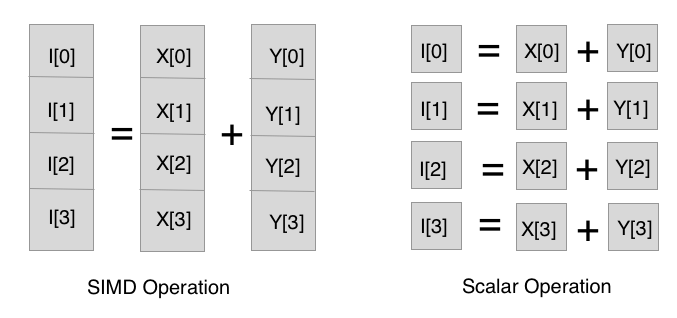
\includegraphics[width=10cm]{pictures/SIMD}
	\caption{Comparison of SIMD and Scalar Operation}
	%\label{fig3.1}  %Reihenfolge ist wichtig! Immer erst \caption{} dann \label{}
\end{figure}

\textit{Fused Multiply-Add (FMA)}\\
FMA is a technique that performs 2 floating-point operations (add and multiply) in one cycle. For example, FMA calculates an entire expression $X + (Y*Z)$ and rounds the final result to $N$ significant bits.  However, an unfused multiply-add would calculate $Y*Z$ and round it to $N$ significant bits. Then it adds the result to $X$ and round it to $N$ significant bits. 

For programs that calculate matrix multiplications, the adds and multiplies are often balance. However, some applications that solve PDEs on structured grids may be dominated by adds with very few multiplies \cite{12}. Those applications do not utilise FMA well. Their attainable performances are worse than those who are entirely dominated by FMA \cite{12}. Therefore, the red line in Figure 3.2(b) represents the computational ceiling for applications that do not utilise FMA. It is below the peak ceiling.\\
In conclusion, applications that do not utilise FMA or SIMD performs worse than others and have lower computational ceilings and smaller machine balances compared to others. 


\section{Time Interval Analysis}

\subsection{Memory Latency}
The memory latency is the delay between the CPU initiates a request until the data is received by the CPU. When the memory controller sends a request for a chunk of data, the upper-level cache L1 is first searched, if a cache miss occurs,  the processor continues to search lower level caches and finally the DRAM. The DRAM then sends the data to the CPU. The Roofline model assumes that there is perfect overlaps of the data transfer and computation because modern processors have several methods to reduce memory latency such as Out-of-Order execution and prefetching. 


\textit{Out-of-Order Execution (OoOE)}\\
In OoOE processor, instructions are stored into a buffer after being fetched and decoded \cite{13}. When the resources and execution units are available, the instruction will be assigned to the unit and then executed. The instructions do not have to be executed in a sequential manner any longer since they can leave the buffer before the older instructions. 

Modern processors operate many times faster than memory. Therefore, in an in-order execution processor, it costs several cycles in a pipeline stage to wait for the data to arrive. The processor has to stall and thus wastes all those cycles. OoOE processors, on the other hand, utilise those cycles to execute other instructions. As a result, it reduces the stalling time of the CPU. 

\begin{figure} [h] %hier können noch Positionierungswünsche angegeben werden
	\centering   % Alles weitere zentrieren
	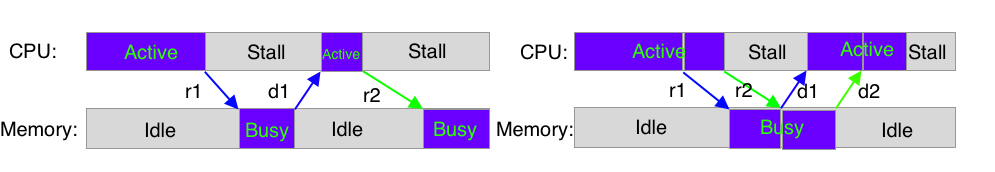
\includegraphics[width=15cm]{pictures/fig3.6}
	\caption{Comparison of in-order execution and OoOE}
	\label{fig3.5}  %Reihenfolge ist wichtig! Immer erst \caption{} dann \label{}
\end{figure}

Figure 3.4 illustrates the processor and memory activities during runtime. The figure on the left side shows the in-order execution. Assuming that we observe the activities in a certain time interval, the processor is proceeding with tasks at the beginning while the memory is idling because there are not any data requests. The processor then sends a data request $r1$ to the memory and begins to stall. The memory starts to read the data. Then it sends the data to the processor ($d1$) and returns to the idle state afterwards. The processor begins to proceed with the instruction. After the instruction is finished, the processor fetches and decodes the next one and then sends another data request $r2$. In this case, there are no overlaps between processor and memory. Therefore, the Roofline model cannot be applied here.

The figure on the right side shows the activities of the OoOE processor and memory. The only difference is that after sending the first data request $r1$, the processor searches the instruction queue to find an instruction whose resources and functional units are available. If there exists such an instruction, it will be executed. The processor may have another instruction that needs data from the memory. As a result, it sends another request $r2$. When the data  arrives ($d1$), the processor executes the first instruction. After finishing the first instruction, the processor immediately begins proceeding with the second one since the data $d2$ arrives.  The processor's stalling time is reduced compared to the in-order execution. However, there is still part of memory latency that cannot be hidden, that is the time for synchronisation between the CPU and memory.  It consists of the memory requests $r1, r2$ and data transfers $d1, d2$. Those time is defined as \textit{transfer delay}.

\textit{Multi-Level Cache and Prefetching}\\
Another technique to reduce memory latency is prefetching. Cache prefetching ensures that the processor fetches the data from DRAM to cache before it is actually needed \cite{14}. The higher the cache level, the faster the data transfer speed from cache to ALU, and thus prefetching allows the processor to reduce memory latency. There are two types of prefetching namely hardware prefetching and software prefetching. Hardware prefetching is realised by hardware prefetchers inside the processor. It monitors the data streams and prefetches the data that the current program might need into the cache without programmer intervention. Software prefetching on the other hand, requires programmer to insert instructions into the program to fetch the required data early \cite{15}. In this work, the focus is on hardware prefetching since I do not modify the source codes of the benchmarks. Figure 3.5 shows the activities of the processor and memory when the hardware prefetching is enabled. Assuming that the processor initiates hardware prefetching at the beginning, the memory becomes busy at the beginning accordingly. In this way, the system realises the overlap of computation and communication. 
\begin{figure} [h] %hier können noch Positionierungswünsche angegeben werden
	\centering   % Alles weitere zentrieren
	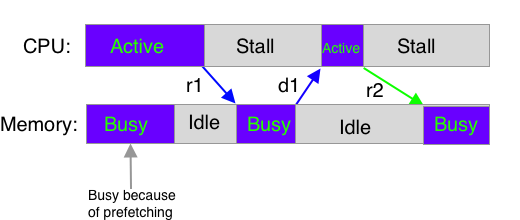
\includegraphics[width=9cm]{pictures/fig3.7}
	\caption{Hardware prefetching}
	\label{fig3.7}  %Reihenfolge ist wichtig! Immer erst \caption{} dann \label{}
\end{figure}

\subsection{Time Interval Analysis}

\begin{table} %[htbp] %hier können noch Positionierungswünsche angegeben werden
	\centering      % Alles weitere zentrieren
	\begin{tabular}{|c|c|} %Alle Spalten zentrieren, ansonsten 'r' oder 'l'
		\hline
		\textbf{Variable} & \textbf{Description}  \\
		\hline
		$T^{active}_{cpu}$               &total time when CPU is active                  \\
		\hline
		$T^{stall}_{cpu}$,	              & total time when CPU is idle              \\
		\hline
		$T^{busy}_{mem}$			& total time when memory is busy\\
		\hline				
		$T^{idle}_{mem}$				& total time when memory is idle\\
		\hline
		$fc$									& core frequency\\
		\hline
		$fuc$								& uncore frequency\\
		\hline
		$CORE\_STEP\_FREQ$  & core step frequency that changed every sampling interval\\
		\hline
		$UNCORE\_STEP\_FREQ$ & uncore step frequency that changed every sampling interval\\
		
		\hline
	\end{tabular}
	\caption{Variables used in this method}
	%\label{tab:vergleich}  %Reihenfolge ist wichtig! Immer erst \caption{} dann \label{}
\end{table}

In many situations the memory latency cannot be eliminated completely. If the Roofline model is directly applied, the total execution time that is calculated in Equation 3.1 will no longer be accurate since the data transfer and computation are not fully overlapped. Therefore, it is important to derive the transfer delay, which is a part of memory latency that cannot be hidden.  This subsection introduces the \textit{time interval analysis},  a method that determines the transfer delay. Table 3.1 describes the variables used in this method.




\subsubsection{Finding the Transfer Delay}

To find the transfer delay, the activities of both processor and memory are observed simultaneously in a time interval. Figures 3.6 and 3.7 represent the situations that the transfer delay is present. Figures 3. 8 and 3.9 show the situations that do not contain transfer delay. The following subsections discuss both situations in detail.

\textbf{With Transfer Delay}
\begin{figure} [h] %hier können noch Positionierungswünsche angegeben werden
	\centering   % Alles weitere zentrieren
	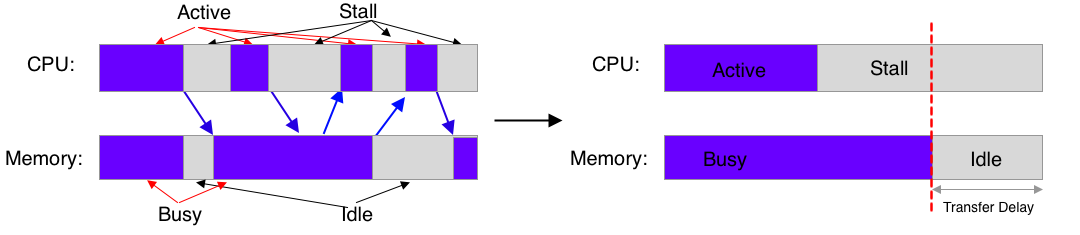
\includegraphics[width=16cm]{pictures/fig3.10}
	\caption{Real time activities vs. summarised activities of memory dominated application with transfer delay}
	\label{fig3.10}  %Reihenfolge ist wichtig! Immer erst \caption{} dann \label{}
\end{figure}
\begin{figure} [h] %hier können noch Positionierungswünsche angegeben werden
	\centering   % Alles weitere zentrieren
	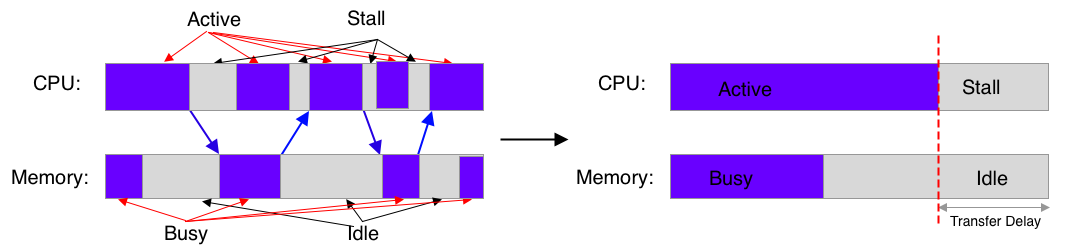
\includegraphics[width=16cm]{pictures/fig3.11}
	\caption{Real time activities vs. summarised activities of computation dominated application with transfer delay}
	\label{fig3.11}  %Reihenfolge ist wichtig! Immer erst \caption{} dann \label{}
\end{figure}

The performance is bound to transfer delay when neither the processor is $100\%$ occupied nor the memory is $100\%$ busy in the time interval. Figure 3.6 and Figure 3.7 show such situations. The figures on the left side of Figure 3.6 and Figure 3.7 illustrate the activities of the processor and memory in real-time. The processor is active for fetching, decoding, and executing instructions. The processor stalls after sending a memory request until the data is transferred to it. The arrows from the CPU to memory are memory requests and the arrows from the memory to the CPU are data transfers. 

In reality, it is hard to measure when exactly the processor is active or stalling. As a result, the right side of Figure 3.6 and Figure 3.7 illustrates the summarised activities. They measure both the active and stalling time of the processor in total and show the proportion of active and stalling time in the figure. Similarly, the total time when the memory is busy and the total time when it is idling are also measured. In this way, it is easier to both measure the data and to exhibit the results. 

The time that the CPU stalls can be derived from the hardware counters with Linux perf. The CPU's active time can be calculated by the time interval minus the CPU's stalling time. The time when memory is busy is calculated via
\begin{equation}
T^{busy}_{mem} = memVolum/Full_{BW}
\end{equation}, where the $memVolum$ is the total amount of data transfer that happens in the time interval and $Full_{BW}$ is the memory bandwidth under the current uncore frequency. The rest of the time interval for memory is idle. 


\newtheorem*{theorem*}{Theorem}
\begin{theorem*}
The transfer delay is $min\{T^{stall}_{cpu}, T^{idle}_{mem}\}$
\end{theorem*}


The transfer delay consists of the time of the memory requests and data transfer. It happens in the synchronisation of the CPU and memory. During the synchronisation, the CPU is not processing any tasks and the memory is not reading or writing any data. Therefore, the transfer delay can be characterised as the time when the memory is idle and the CPU stalls simultaneously. In Figure 3.6, the transfer delay approximates to $T^{idle}_{mem}$ while in Figure 3.7 to $T^{stall}_{cpu}$. Combining two situations, the transfer delay approximates to $min\{T^{stall}_{cpu}, T^{idle}_{mem}\}$.



\textbf{Without Transfer Delay}

\begin{figure} [h] %hier können noch Positionierungswünsche angegeben werden
	\centering   % Alles weitere zentrieren
	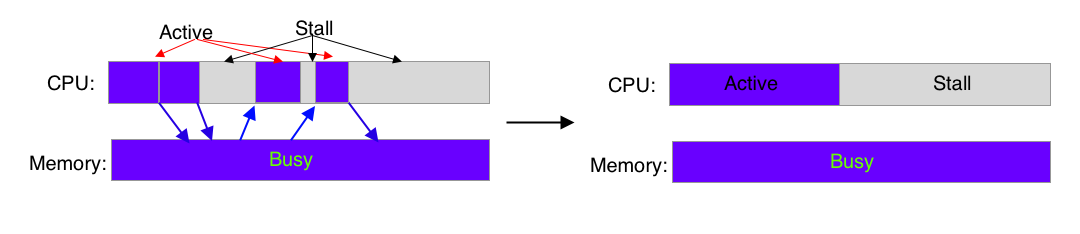
\includegraphics[width=16cm]{pictures/fig3.8}
	\caption{Real time activities vs. summarised activities of memory bound application}
	\label{fig3.8}  %Reihenfolge ist wichtig! Immer erst \caption{} dann \label{}
\end{figure}
\begin{figure} [h] %hier können noch Positionierungswünsche angegeben werden
	\centering   % Alles weitere zentrieren
	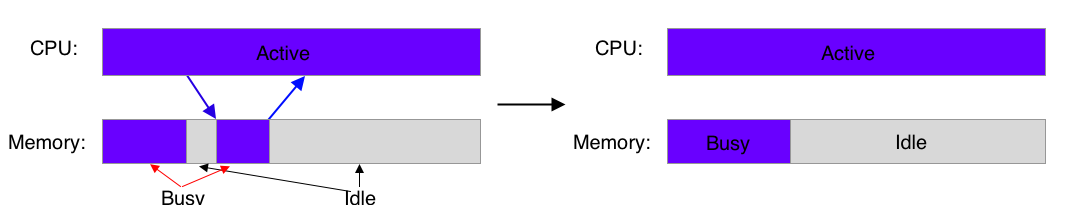
\includegraphics[width=16cm]{pictures/fig3.9}
	\caption{Real time activities vs. summarised activities of compute bound application}
	\label{fig3.9}  %Reihenfolge ist wichtig! Immer erst \caption{} dann \label{}
\end{figure}
Similar to Figures 3.6 and 3.7, Figures 3.8 and 3.9 present the real-time activities on the left and the summarised activity's time on the right. Neither of the situations contains a time slot where the memory is idle and the CPU stalls simultaneously. According to Theorem, the transfer delay approximates to $0$. The Roofline model can be applied here to determine whether it is compute-bound or memory-bound.



